\chapter{约束满足问题}

\section{约束满足问题}

\subsection{约束满足问题(CSP, Constraint Satisfaction Problems)}

在CSP问题中,存在一组变量,当每个变量都被赋了一个值,且能够满足所有的约束条件时,问题就解决了。\\

CSP问题包含:

\begin{itemize}
    \item $ X = \{X_1, X_2, \cdots, X_n\} $:变量集合
    \item $ D = \{D_1, D_2, \cdots, D_n\} $:域(domain)
    \item $ C $:约束集合
\end{itemize}

约束可分为:

\begin{itemize}
    \item 一元约束(unary constraint):只对一个变量进行约束,如$ A \neq 3 $、$ B \neq 4 $。
    \item 二元约束(binary constraint):对两个变量进行约束,如$ A < B $、$ B < C $。
    \item 多元约束:对两个以上的变量进行约束,如$ A + B < C $。
\end{itemize}

例如$ X = \{A, B, C\} $,$ dom(A) = dom(B) = dom(C) = \{1, 2, 3, 4\} $,约束条件为$ A < B $和$ B < C $。\\

其中$ A = 2 $、$ B = 3 $、$ C = 4 $是一组满足要求的赋值,而$ A = 2 $、$ B = 3 $、$ C = 1 $就是一组不满足要求的赋值。\\

\subsection{澳大利亚地图着色问题}

在澳大利亚地图着色问题中,

\begin{itemize}
    \item $ X = \{WA, NT, SA, Q, NSW, V, T\} $
    \item $ D = \{Red, Green, Blue\} $
    \item $ C = \{SA \neq WA, SA \neq NT, SA \neq Q, SA \neq V, SA \neq NSW, WA \neq NT, NT \neq Q, Q \neq NSW, NSW \neq V\} $
\end{itemize}

\begin{figure}[H]
    \centering
    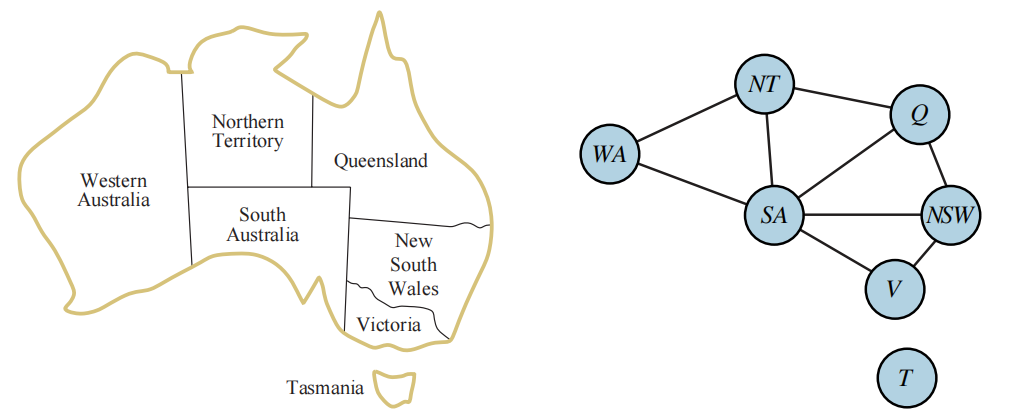
\includegraphics{img/C2/2-1/1.png}
\end{figure}

\begin{figure}[H]
    \centering
    \begin{tikzpicture}
        \begin{scope}[every node/.style={circle,thick,draw}]
            \node (NT) at (-1.5,2) {NT};
            \node (Q) at (1.5,2) {Q};
            \node (WA) at (-4,0) {WA};
            \node (SA) at (0,0) {SA};
            \node (NSW) at (4,0) {NSW};
            \node (V) at (1.5,-2) {V};
            \node (T) at (1.5,-4) {T};
        \end{scope}

        \begin{scope}[>={Stealth[black]},
            every node/.style={},
            every edge/.style={draw=black,very thick}]
            \path [-] (NT) edge node {} (Q);
            \path [-] (NT) edge node {} (SA);
            \path [-] (Q) edge node {} (SA);
            \path [-] (Q) edge node {} (NSW);
            \path [-] (WA) edge node {} (NT);
            \path [-] (SA) edge node {} (WA);
            \path [-] (SA) edge node {} (NSW);
            \path [-] (SA) edge node {} (V);
            \path [-] (NSW) edge node {} (V);
        \end{scope}
    \end{tikzpicture}
    \caption{澳大利亚地图}
\end{figure}

\vspace{0.5cm}

\subsection{密码算术谜题}

在密码算术谜题中,每个字母代表一个不同的数字。

\begin{table}[H]
    \centering
    \begin{tabular}{cD{.}{.}{3}}
          & TWO  \\
        + & TWO  \\
        \hline
        = & FOUR
    \end{tabular}
\end{table}

\begin{itemize}
    \item 变量
          \begin{itemize}
              \item $ X = \{T, W, O, F, U, R, C_1, C_2, C_3\} $,其中$ C_1 $、$ C_2 $、$ C_3 $为进位。
          \end{itemize}
    \item 域
          \begin{itemize}
              \item $ dom(T) = dom(W) = dom(O) = dom(F) = dom(U) = dom(R) = \{0, 1, \cdots, 9\} $
              \item $ dom(C_1) = dom(C_2) = dom(C_3) = \{0, 1\} $
          \end{itemize}
    \item 约束
          \begin{itemize}
              \item $ AllDiff(T, W, O, F, U, R)  $
              \item $ O + O = R = 10C_1 $
              \item $ C_1 + W + W = U + 10C_2 $
              \item $ C_2 + T + T = O + 10C_3 $
              \item $ C_3 = F $
              \item $ T \neq 0 $
              \item $ F \neq 0 $
          \end{itemize}
\end{itemize}

\vspace{0.5cm}

\subsection{数独}

数独的目标是在$ 9 \times 9 $的方格中填入数字,使得每一行、每一列和每一个$ 3 \times 3 $的小方格中都包含$ 1 \sim 9 $的数字。\\

\begin{sudoku}
    | | |3| |2| |6| | |.
    |9| | |3| |5| | |1|.
    | | |1|8| |6|4| | |.
    | | |8|1| |2|9| | |.
    |7| | | | | | | |8|.
    | | |6|7| |8|2| | |.
    | | |2|6| |9|5| | |.
    |8| | |2| |3| | |9|.
    | | |5| |1| |3| | |.
\end{sudoku}

假设数独的行号为$ A \sim I $,列号为$ 1 \sim 9 $。

\begin{itemize}
    \item 变量
          \begin{itemize}
              \item $ X = \{A1, \cdots, A9, B1, \cdots \cdots, I1, \cdots I9\} $
          \end{itemize}
    \item 域
          \begin{itemize}
              \item $ D = \{1, 2, 3, 4, 5, 6, 7, 8, 9\} $
          \end{itemize}
    \item 约束
          \begin{itemize}
              \item $ AllDiff(A1, A2, A3, A4, A5, A6, A7, A8, A9) $
              \item $ AllDiff(B1, B2, B3, B4, B5, B6, B7, B8, B9) $
              \item $ \cdots $
              \item $ AllDiff(A1, B1, C1, D1, E1, F1, G1, H1, I1) $
              \item $ AllDiff(A2, B2, C2, D2, E2, F2, G2, H2, I2) $
              \item $ \cdots $
              \item $ AllDiff(A1, A2, A3, B1, B2, B3, C1, C2, C3) $
              \item $ AllDiff(A4, A5, A6, B4, B5, B6, C4, C5, C6) $
              \item $ \cdots $
          \end{itemize}
\end{itemize}

\newpage

\section{约束传播}

\subsection{弧相容(Arc Consistency)}

约束传播(Constrain Propagation)的目的是减少变量的合法取值,有时如果所有变量的域都被减少为1时,它可以直接算出结果。约束传播还可以检测失败的情况,当某一个变量的域被减少为0时,该问题将无解。\\

如果变量$ X_i $的域$ D_i $中的每个值都满足在变量$ X_j $的域$ D_j $中的值时,称$ X_i $和$ X_j $是弧相容的。\\

例如:

\begin{itemize}
    \item 变量:$ X, Y $
    \item 域:$ dom(X) = dom(Y) = \{1, \cdots, 9\} $
    \item 约束:$ Y = X^2 $
\end{itemize}

当变量$ X $取$ \{4, 5, 6, 7, 8, 9\} $时,$ X $与$ Y $不满足弧相容。\\

当变量$ Y $取$ \{2, 3, 5, 6, 7, 8\} $时,$ Y $与$ X $不满足弧相容。\\

为了让$ X $和$ Y $都互相满足弧相容,需要从$ dom(X) $和$ dom(Y) $中移除不满足弧相容的值。因此

\vspace{-1cm}

\begin{align*}
    dom(X) = \{0, 1, 2, \cdots, 9\}\ \backslash \ \{4, 5, 6, 7, 8, 9\} = \{0, 1, 2, 3\} \\
    dom(Y) = \{0, 1, 2, \cdots, 9\}\ \backslash \ \{2, 3, 5, 6, 7, 8\} = \{0, 1, 4, 9\}
\end{align*}

AC-3(Arc Consistency-3)算法用于解决CSP问题,早期的AC算法效率太低,而AC-3更为简单常用。\\

\begin{algorithm}[H]
    \caption{AC-3}
    \begin{algorithmic}[1]
        \Procedure{AC-3}{csp} returns false if inconsistency found and true otherwise
        \State queue = [all arcs in csp]
        \\
        \While {not queue.is\_empty()}
        \State $ (X_i, X_j) $ = queue.dequeue()
        \If {Revise(csp, $ X_i $, $ X_j $)}
        \If {size($ D_i $) == 0}
        \State \Return false
        \EndIf
        \For {$ X_k $ in $ X_i $.Neighbors - \{$ X_j $\}}
        \State queue.enqueue($ (X_i, X_j) $)
        \EndFor
        \EndIf
        \EndWhile
        \\
        \State \Return true
        \EndProcedure
        \\
        \Procedure{Revise}{csp, $ X_i $, $ X_j $} returns true iff we revise the domain of $ X_i $
        \State revised = false
        \For {$ x $ in $ D_i $}
        \If {no value $ y $ in $ D_j $ allows (x, y) to satisfy contraint $ (X_i, X_j) $}
        \State delete $ x $ from $ D_i $
        \State revised = true
        \EndIf
        \EndFor
        \State \Return revised
        \EndProcedure
    \end{algorithmic}
\end{algorithm}

\newpage

\section{回溯搜索}

\subsection{回溯搜索(Backtracking Search)}

回溯就是简单粗暴的试错方法。例如走迷宫,大多人类一般就是使用回溯法,当走到一条死路,就往回退到前一个岔路,尝试另外一条,直到走出。\\

回溯搜索与DFS类似,回溯搜索每次为变量选择一个赋值,当没有合法的值可以赋给该变量时就回溯返回,尝试别的路径。\\

\begin{figure}[H]
    \centering
    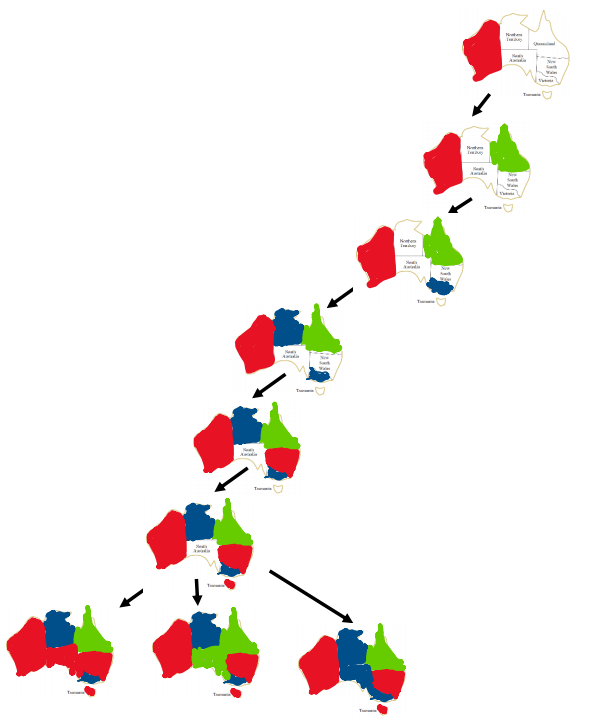
\includegraphics[scale=0.8]{img/C2/2-3/1.png}
    \caption{回溯搜索}
\end{figure}

\begin{algorithm}[H]
    \caption{Backtracking Search}
    \begin{algorithmic}[1]
        \Procedure{BacktrackingSearch}{csp} returns a solution or failure
        \State \Return Backtrack(csp, \{\})
        \EndProcedure
        \\
        \Procedure{Backtrack}{csp, assignment} returns a solution or failure
        \If {assignment is complete}
        \State \Return assignment
        \EndIf
        \\
        \State var = SelectUnassignedVariable(csp, assignment)
        \For {value in OrderDomainValues(csp, var, assignment)}
        \If {value is consistent with assignment}
        \State assignment.add({var = value})
        \State inferences = Inference(csp, var, assignment)
        \If {inferences != failure}
        \State csp.add(inferences)
        \State result = Backtrack(csp, assignment)
        \If {result != failure}
        \State \Return result
        \EndIf
        \State csp.remove(inferences)
        \EndIf
        \State assignment.remove({var = value})
        \EndIf
        \EndFor
        \\
        \State \Return failure
        \EndProcedure
    \end{algorithmic}
\end{algorithm}

\vspace{0.5cm}

\subsection{前向检查(Forward Checking)}

前向检查可用于将还没有进行赋值的候选变量进行适当排除。\\

在澳大利亚地图着色问题中,一开始,所有省份的颜色都能够选择所有域中的颜色。\\

当WA选择了红色后,相邻的NT和SA的颜色域就需要删除红色。当Q选择了绿色后,相邻的NT、NSW和SA的颜色域就需要删除绿色。当V选择了蓝色后,相邻的NSW和SA的颜色域就需要删除蓝色。\\

\begin{figure}[H]
    \centering
    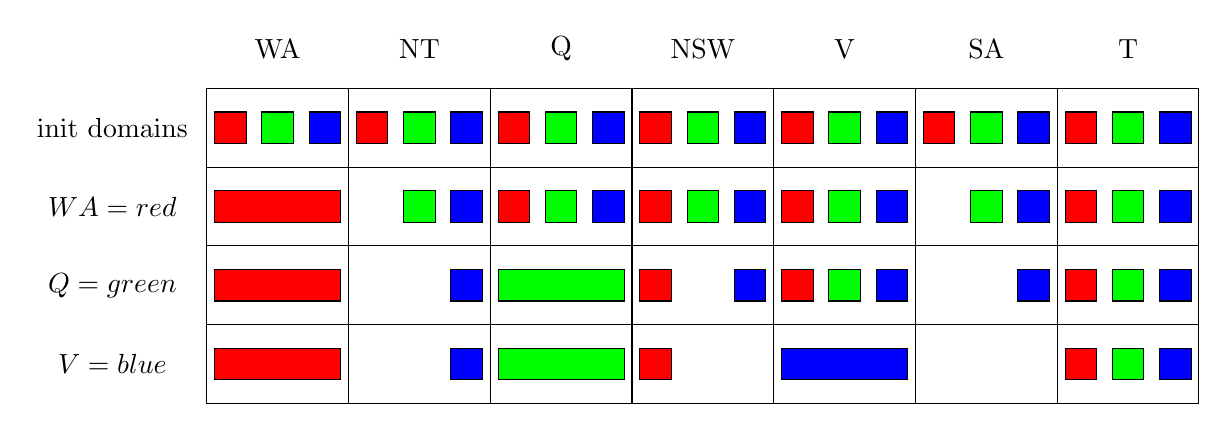
\begin{tikzpicture}
        \draw (0,0) rectangle (12.6,4);
        \draw[-] (1.8,0) -- (1.8,4);
        \draw[-] (3.6,0) -- (3.6,4);
        \draw[-] (5.4,0) -- (5.4,4);
        \draw[-] (7.2,0) -- (7.2,4);
        \draw[-] (9,0) -- (9,4);
        \draw[-] (10.8,0) -- (10.8,4);
        \draw[-] (0,1) -- (12.6,1);
        \draw[-] (0,2) -- (12.6,2);
        \draw[-] (0,3) -- (12.6,3);

        \node at (0.9,4.5) {WA};
        \node at (2.7,4.5) {NT};
        \node at (4.5,4.5) {Q};
        \node at (6.3,4.5) {NSW};
        \node at (8.1,4.5) {V};
        \node at (9.9,4.5) {SA};
        \node at (11.7,4.5) {T};

        \node at (-1.2,3.5) {init domains};
        \node at (-1.2,2.5) {$ WA = red $};
        \node at (-1.2,1.5) {$ Q = green $};
        \node at (-1.2,0.5) {$ V = blue $};

        \draw[-,fill=red] (0.1,3.3) rectangle (0.5,3.7);
        \draw[-,fill=green] (0.7,3.3) rectangle (1.1,3.7);
        \draw[-,fill=blue] (1.3,3.3) rectangle (1.7,3.7);
        \draw[-,fill=red] (1.9,3.3) rectangle (2.3,3.7);
        \draw[-,fill=green] (2.5,3.3) rectangle (2.9,3.7);
        \draw[-,fill=blue] (3.1,3.3) rectangle (3.5,3.7);
        \draw[-,fill=red] (3.7,3.3) rectangle (4.1,3.7);
        \draw[-,fill=green] (4.3,3.3) rectangle (4.7,3.7);
        \draw[-,fill=blue] (4.9,3.3) rectangle (5.3,3.7);
        \draw[-,fill=red] (5.5,3.3) rectangle (5.9,3.7);
        \draw[-,fill=green] (6.1,3.3) rectangle (6.5,3.7);
        \draw[-,fill=blue] (6.7,3.3) rectangle (7.1,3.7);
        \draw[-,fill=red] (7.3,3.3) rectangle (7.7,3.7);
        \draw[-,fill=green] (7.9,3.3) rectangle (8.3,3.7);
        \draw[-,fill=blue] (8.5,3.3) rectangle (8.9,3.7);
        \draw[-,fill=red] (9.1,3.3) rectangle (9.5,3.7);
        \draw[-,fill=green] (9.7,3.3) rectangle (10.1,3.7);
        \draw[-,fill=blue] (10.3,3.3) rectangle (10.7,3.7);
        \draw[-,fill=red] (10.9,3.3) rectangle (11.3,3.7);
        \draw[-,fill=green] (11.5,3.3) rectangle (11.9,3.7);
        \draw[-,fill=blue] (12.1,3.3) rectangle (12.5,3.7);

        \draw[-,fill=red] (0.1,2.3) rectangle (1.7,2.7);
        \draw[-,fill=green] (2.5,2.3) rectangle (2.9,2.7);
        \draw[-,fill=blue] (3.1,2.3) rectangle (3.5,2.7);
        \draw[-,fill=red] (3.7,2.3) rectangle (4.1,2.7);
        \draw[-,fill=green] (4.3,2.3) rectangle (4.7,2.7);
        \draw[-,fill=blue] (4.9,2.3) rectangle (5.3,2.7);
        \draw[-,fill=red] (5.5,2.3) rectangle (5.9,2.7);
        \draw[-,fill=green] (6.1,2.3) rectangle (6.5,2.7);
        \draw[-,fill=blue] (6.7,2.3) rectangle (7.1,2.7);
        \draw[-,fill=red] (7.3,2.3) rectangle (7.7,2.7);
        \draw[-,fill=green] (7.9,2.3) rectangle (8.3,2.7);
        \draw[-,fill=blue] (8.5,2.3) rectangle (8.9,2.7);
        \draw[-,fill=green] (9.7,2.3) rectangle (10.1,2.7);
        \draw[-,fill=blue] (10.3,2.3) rectangle (10.7,2.7);
        \draw[-,fill=red] (10.9,2.3) rectangle (11.3,2.7);
        \draw[-,fill=green] (11.5,2.3) rectangle (11.9,2.7);
        \draw[-,fill=blue] (12.1,2.3) rectangle (12.5,2.7);

        \draw[-,fill=red] (0.1,1.3) rectangle (1.7,1.7);
        \draw[-,fill=blue] (3.1,1.3) rectangle (3.5,1.7);
        \draw[-,fill=green] (3.7,1.3) rectangle (5.3,1.7);
        \draw[-,fill=red] (5.5,1.3) rectangle (5.9,1.7);
        \draw[-,fill=blue] (6.7,1.3) rectangle (7.1,1.7);
        \draw[-,fill=red] (7.3,1.3) rectangle (7.7,1.7);
        \draw[-,fill=green] (7.9,1.3) rectangle (8.3,1.7);
        \draw[-,fill=blue] (8.5,1.3) rectangle (8.9,1.7);
        \draw[-,fill=blue] (10.3,1.3) rectangle (10.7,1.7);
        \draw[-,fill=red] (10.9,1.3) rectangle (11.3,1.7);
        \draw[-,fill=green] (11.5,1.3) rectangle (11.9,1.7);
        \draw[-,fill=blue] (12.1,1.3) rectangle (12.5,1.7);

        \draw[-,fill=red] (0.1,0.3) rectangle (1.7,0.7);
        \draw[-,fill=blue] (3.1,0.3) rectangle (3.5,0.7);
        \draw[-,fill=green] (3.7,0.3) rectangle (5.3,0.7);
        \draw[-,fill=red] (5.5,0.3) rectangle (5.9,0.7);
        \draw[-,fill=blue] (7.3,0.3) rectangle (8.9,0.7);
        \draw[-,fill=red] (10.9,0.3) rectangle (11.3,0.7);
        \draw[-,fill=green] (11.5,0.3) rectangle (11.9,0.7);
        \draw[-,fill=blue] (12.1,0.3) rectangle (12.5,0.7);
    \end{tikzpicture}
    \caption{前向检查}
\end{figure}

此时发现,SA的颜色域为空,说明当前的选择不合法,需要回溯。\\

\subsection{变量和取值顺序}

变量和取值顺序可以对回溯搜索进行优化,从而减少搜索空间。\\

一个常用的选择标准是最小剩余值(Minimum Remaining Values),也就是选择域中包含选择最少的变量。在每次给当前的变量赋值之后,其它变量的域可能会更新,那么包含元素最少的变量,就代表这个变量的域可能最早变为空,从而产生死结点。\\

最小剩余值的排序方法认为,既然问题迟早可能暴露,那就选择一种可以让问题尽早暴露的方式。这种方式也被称为Fail-First。\\

最小剩余值是基于变量进行选择的,而另一种最小约束值(Least Constraining Value)讨论的是当一个变量被选定时,从其域中选择哪个值的方式。\\

最少约束值优先选择的值应该试图为剩余变量赋值留下最大的空间。因为在CSP问题中,无论如何都要对所有的变量进行值的分配,因此必须把困难的变量情况放在前面进行讨论,这样可以提前暴露问题,触发回溯行为,避免不必要的计算。但是对于每个变量的值的选择来说,并不是每个值都会用到,因此只需要选择最有效的值即可。\\

\newpage

\section{CSP局部搜索}

\subsection{CSP局部搜索}

回溯搜索从一个空的初始状态开始,逐个尝试对变量赋值,当选择不合法时就进行回溯,因此回溯搜索始终保持弧相容。\\

局部搜索算法对求解许多CSP都是很有效的,它从一个完整地随机布局开始,这个初始布局有可能会违反约束,局部搜索的目的就是消除这些矛盾。在为变量选择新值的时候,最明显的启发式是选择与其它变量冲突最少的值。\\

\begin{algorithm}[H]
    \caption{MinConflicts}
    \begin{algorithmic}[1]
        \Procedure{MinConflicts}{csp, max\_steps} returns a solution or failure
        \State current = an initial complete assignment for csp
        \For {i = 1 to max\_steps}
        \If {current is a solution for csp}
        \State \Return current
        \EndIf
        \State var = a randomly chosen conflicted variable from csp.Variables
        \State value = the value v for var that minimizes Conflicts(csp, var, v, current)
        \State current.update({var = value})
        \EndFor
        \State \Return failure
        \EndProcedure
    \end{algorithmic}
\end{algorithm}

\newpage